\documentclass[10pt]{article}
\usepackage[a4paper,bottom=3cm]{geometry}
\usepackage[english]{babel}
\usepackage[utf8]{inputenc}
\usepackage{amsmath}
\usepackage{amsthm}
\usepackage{amssymb}
\usepackage{graphicx}
\usepackage{subfig}
\usepackage{hyperref}

\theoremstyle{definition}
\newtheorem{definition}{Definition}[section]

\author{Takudzwa Togarepi, Julian Bopp }
\title{Project Part 1: Probabilistic modeling of the femur anatomy}
\begin{document}

\maketitle

\begin{abstract}
\noindent
The femur bone is a crucial part of the human anatomy used in forensic science due to its size and strength. It can provide valuable insights into the gender and geographical origin of the person whose remains are being analyzed. This is because femurs of people with similar geographical origin or of the same gender tend to be similar. However it is likely that when examining human remains we only get a partial or deformed femur, this is where we would need femur reconstruction to model what the full femur would have looked like and analyze it. In this project we came up with a model which we would use to reconstruct given partial femurs. We also analyzed and validated our model using statistical approaches.\\

\noindent
$\bold{Keywords}$: femur, forensics, gender determination, reconstruction, modeling.
\end{abstract}
\section{Introduction}
The main goal of this project is to develop a probabilistic shape model for femur bones.
Femur bone reconstruction is an important task in the field of forensics as it can aid in the human identification just by analyzing the femur bones from the human remains . In this paper, we present an approach to develop a probabilistic shape model for femur bones using a combination of rigid alignment, Gaussian Process modeling, Iterative Closest Points (ICP), and Principal Component Analysis(PCA).\\

\noindent
In our approach we used a dataset of femur meshes and femur landmarks, comprising 47 samples each. We first applied rigid alignment, followed by building a Gaussian Process model(GP-model) to capture the shape variation of the femur bones. We then used an iterative alignment refinement technique called ICP to fit the GP-model by aligning the femur meshes with the model.\\

\section{Methods}
%In this section you can describe the methods you used to solve the problem.
In this section we describe the necessary mathematical background and the assumptions that we make for our model. We assume a reference shape with point set $\Gamma_R$. Instead of modelling the shape directly, we model the possible deformations. Let $x\in\Gamma_R$, we assume that the deformation $u(x)$ of $x$ follows a normal distribution. We know assume that we have a mean function $\mu$ and a covariance function $k$ that map each point of $\Gamma_R$ to their mean deformation and each pair of points of $\Gamma_R$ to their joint distribution covariance matrix, respectively.

\begin{definition}[Gaussian Process)]
A Gaussian process $\mu \sim N(\vec{\mu},K)$ is defined on a finite point set $\Gamma_R$
with
\begin{align}\label{eq:1}
\vec{\mu} &= \left(\mu(x)\right)_{x\in\Gamma_R}\\
        K &= \left(k(x,x')\right)_{x,x'\in\Gamma_R},\label{eq:2}
\end{align}
It is also written as $u\sim GP(\mu,k)$ and the definition can be extended to arbitrary sets $\Gamma_R$.
\end{definition}
A common kernel is the Gaussian kernel
\begin{definition}[Gaussian kernel]
\begin{equation}\label{eq:gausskernel}
k(x,x') = s\ e^{(-(x-x')^2/l)}
\end{equation}

\end{definition}


If we have data that is in correspondence (for every point on one shape we can identify the corresponding point on the other shapes), then we can superimpose them and use maximum likelihood estimators to learn a suitable mean and covariance function for our Gaussian process. Assuming $n$ shapes with $u^i,\ i=1,\dots,n$ as their deformation field these estimators are
\begin{align}
\hat\mu(x) &= \frac{1}{n}\sum_{i=1}^n u^i(x)\label{eq:3}\\
\hat k(x,x') = \frac{1}{n-1}\sum_{i}^n &(u^i(x) - \mu(x))(u^i(x') - \mu(x'))^\top.\label{eq:4}
\end{align}
Whenever we create a sample of a Gaussian process using the estimators of \eqref{eq:3} and \eqref{eq:4} we
would have to store a matrix of size $Nd \times Nd$, where $N$ denotes the number of points of the shape and $d$ the dimensionality of the output space (in case of 3D objects like our femur data, $d=3$). This results in a huge matrix that is not feasible to store. Luckily there is a solution to this problem.

\begin{definition}[Karhunen-Loève expansion in the discrete case]
Let $u \sim GP(\mu,k)$ be a discrete Gaussian process using the estimators \eqref{eq:3} and \eqref{eq:4}. Then
\begin{equation}
\hat u = \mu + \sum_{i=1}^n \sqrt{d_i}\vec{\varphi}_i\hat \alpha_i,\, \hat \alpha_i\sim N(0,1)
\end{equation}
where $\vec{\varphi}_i$ and $d_i$ are the $i$-th eigenvector and eigenvalue of $K$, respectively.
\end{definition}
\noindent
Using this expansion we can calculate a low-rank approximation (cut off the sum after some point) of the Gaussian process.

Since the given data is not in correspondence we use iterative closest points (ICP) and GP regression to approximate the correspondence. We used the implementation from \href{https://scalismo.org/docs/Tutorials/tutorial11}{Tutorial11}.




\newpage
\section{Experiments and results}
\subsection{Data and experimental setup}

%Explain the data with which you are experimenting.
%Highlight aspects of the data that are particularly interesting
%for the project.

The data on which we are experimenting consists of 47 femurs. Included in this data are landmarks $L0,\dots,L5$ for every femur. The data is not completely in correspondence, but the landmarks are. We therefore align the data using rigid alignment on the landmarks.
In particular $L3,L4$, as seen in figure \ref{fig:landmark_width}, can be used to estimate the width of the femur, whereas $L2,L5$, as seen in figure \ref{fig:landmark_length}, can be used to estimate the length.

\begin{figure}[h]
\centering
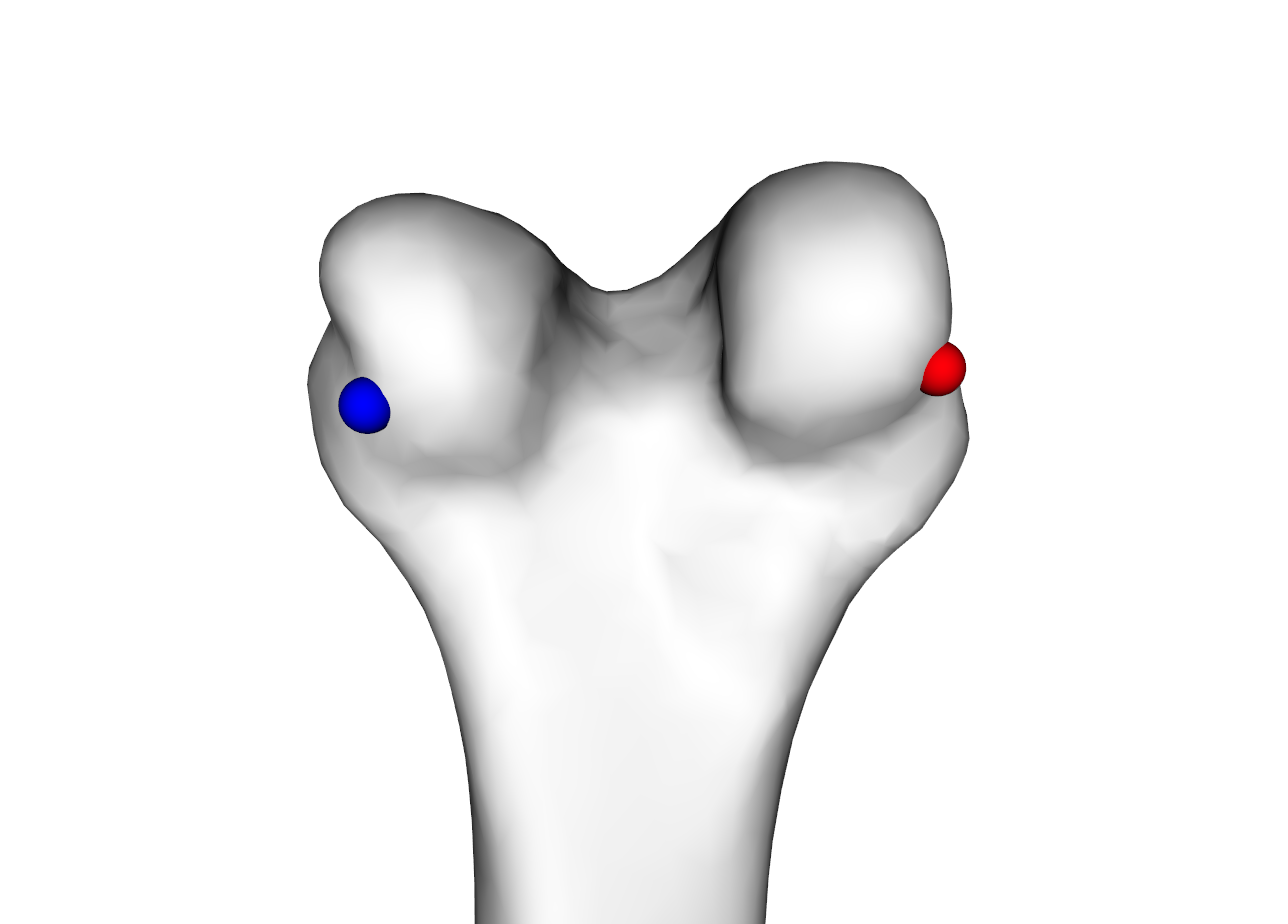
\includegraphics[scale=0.2]{screenshots/length_L3red_L4blue.png}
\caption{Landmark $L3$ in red, and landmark $L4$ in blue. Used to estimate the width of the femur bone.}
\label{fig:landmark_width}
\end{figure}

\begin{figure}[h]
\centering
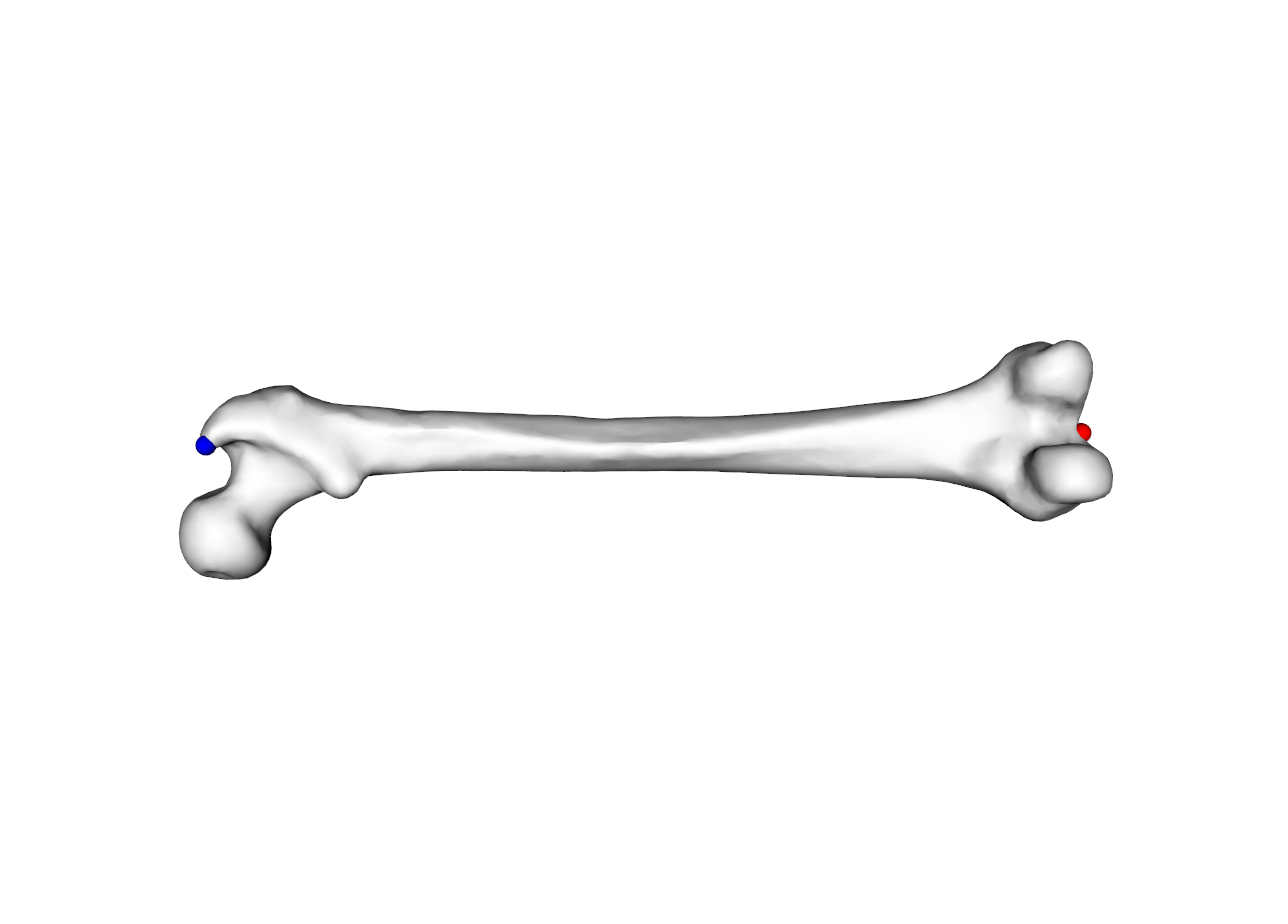
\includegraphics[scale=0.2]{screenshots/width_L2blue_L5red.png}
\caption{Landmark $L3$ in blue, and landmark $L4$ in red. Used to estimate the length of the femur bone.}
\label{fig:landmark_length}
\end{figure}
\noindent
To estimate the length of a femur we calculate the distance between the $L2$ and $L5$ landmark, similarly we estimate the width by calculating the distance between the $L3$ and $L4$ landmark. We display the measurements made from the 47 femurs in figure \ref{fig:scatterplot_femurdata} and summarize them in table \ref{table:mean_variance_femur_data} by calculating the mean and variance.
\begin{figure}
\centering
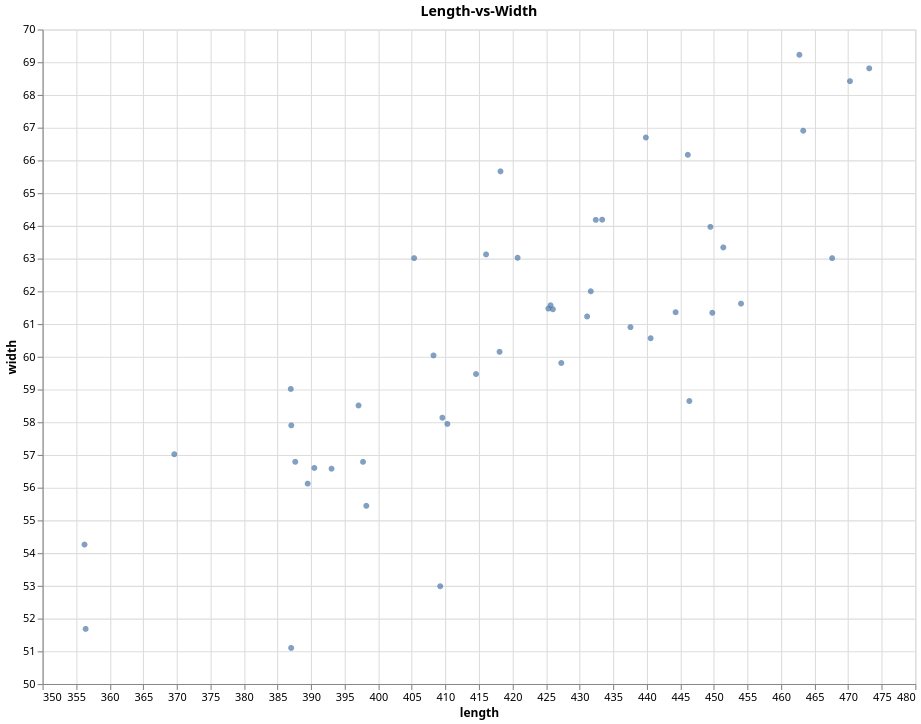
\includegraphics[scale=0.35]{screenshots/data_scatterplot.png}
\caption{Scatterplot of calculated length and width of the femur data}
\label{fig:scatterplot_femurdata}
\end{figure}
\begin{table}[h!]
\centering
\begin{tabular}{c|r|r}
 & Mean & Variance \\
\hline
Length & 420.80 & 841.94 \\
Width & 60.61 & 18.13
\end{tabular}
\caption{Mean and variance of length and width of the femur data.}
\label{table:mean_variance_femur_data}
\end{table}

We notice a high variability of the data. This gives reason to believe that the 47 femur samples are not from subjects that all share similar femurs. More precisely, the data probably originates from males and females with a large variability in height, and therefore, a large variability in femur length and width. Visually, figure \ref{fig:scatterplot_femurdata} gives reason to believe that the length and width are correlated. There is a trend that shows that an increase in length comes with an increase in width.

In our experiment we create a Statistical Shape Model (SSM) that allows us to take random samples which look like actual femurs. To validate the model, we take the same measurements as with the data, i.e. we calculate the distance between the landmark pairs that estimate width and length of a femur, and compare them. Ideally the measurements of the mean and variance of the length and width of our model should be similar to those measurements of the actual data. Moreover the correlation between length and width as seen in figure \ref{fig:scatterplot_femurdata} should be adopted by the model samples. Additionally we make visual checks of the model generated samples to make sure that they do not overly produce shapes that do not like a femur bone. To setup our model we went through the following steps
\begin{itemize}
\item
We start with a basic Gaussian process based on a sample reference femur with zero mean and a matrix valued Gaussian kernel. The Gaussian kernel is the result of three one dimensional Gaussian kernels \eqref{eq:gausskernel} each placed on one position of the diagonal. The parameters used for the kernels where $s_x= 5\ l_x= 50, s_y=5\ l_y=50, s_z=20 \ l_z = 200$. Picking a larger value for $s_z$ made sure that the length variations were more extreme compared to the width variations.
\item We used the ICP algorithm to find parameters of our basic model that best fit the shape of the 47 femurs of our dataset. The resulting model samples are in correspondence.
\item Using \eqref{eq:3} and \eqref{eq:4} we were able to find a better mean and covariance that more closely describes the data.
\item In a last step we enlarge the flexibility of our model by augmenting the kernel with an additional Gaussian kernel.

\end{itemize}

\subsection{Experimental results}
Using the basic Gaussian process based on a single reference femur we get mean measurements that closely resemble the measurements of the single reference femur, which is to be expected. However, the choice of parameters of the kernel results in a variance (table \ref{table:mean_variance_analyticalgp}) that is comparable to the measurements of the actual data in table \ref{table:mean_variance_femur_data}. Since the kernel used is a diagonal one, we don't have any correlation between length and width, as seen in
figure \ref{fig:scatterplot_analyticalgp}.

\begin{figure}[h!]
\centering
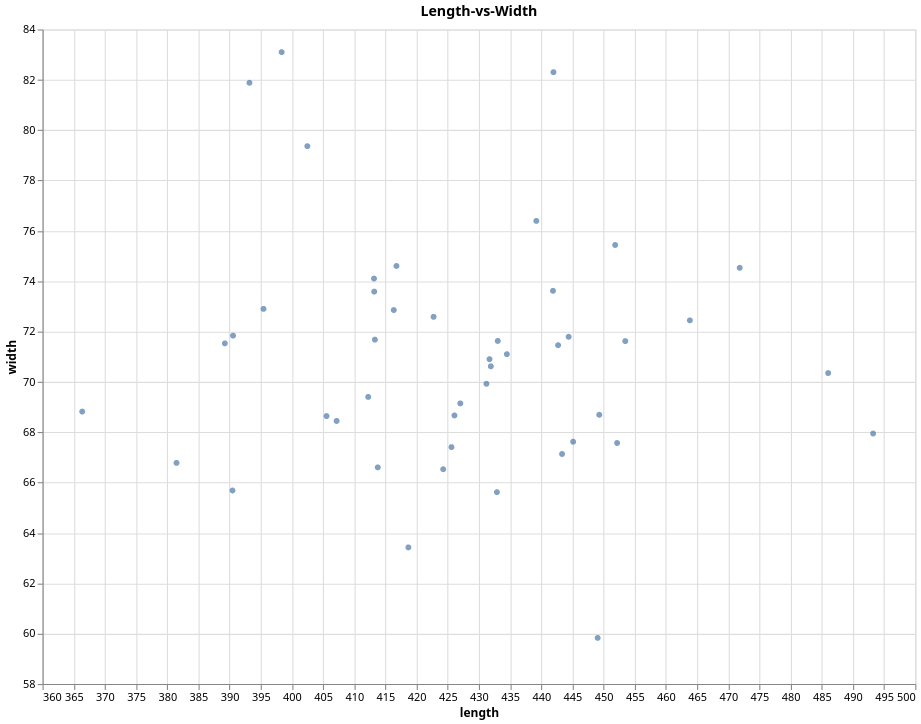
\includegraphics[scale=0.35]{screenshots/analyticalgp_scatterplot.png}
\caption{Scatterplot of calculated length and width of 47 samples from an analytical Gaussian process using a single reference femur.}
\label{fig:scatterplot_analyticalgp}
\end{figure}
\begin{table}[h!]
\centering
\begin{tabular}{c|r|r}
 & Mean & Variance \\
\hline
Length & 426.70 & 687.57 \\
Width & 71.05 & 21.01
\end{tabular}
\caption{Mean and variance of length and width of 47 samples from an analytical Gaussian process using a single reference femur.}
\label{table:mean_variance_analyticalgp}
\end{table}

Next, using ICP, learning the mean and covariance data with \eqref{eq:3} and \eqref{eq:4}, and augmenting the kernel with a Gaussian kernel, we took the following measurements presented in table \ref{table:mean_variance_fitted_augmented}. The measurements closely resemble those of the actual data, but we notice that the mean width is slightly too high. Moreover we can see in figure \ref{fig:scatterplot_fitted_augmented} that the samples from the fitted+augmented model exhibit a correlation of length and width similar to that of the real data.
\begin{figure}[h!]
\centering
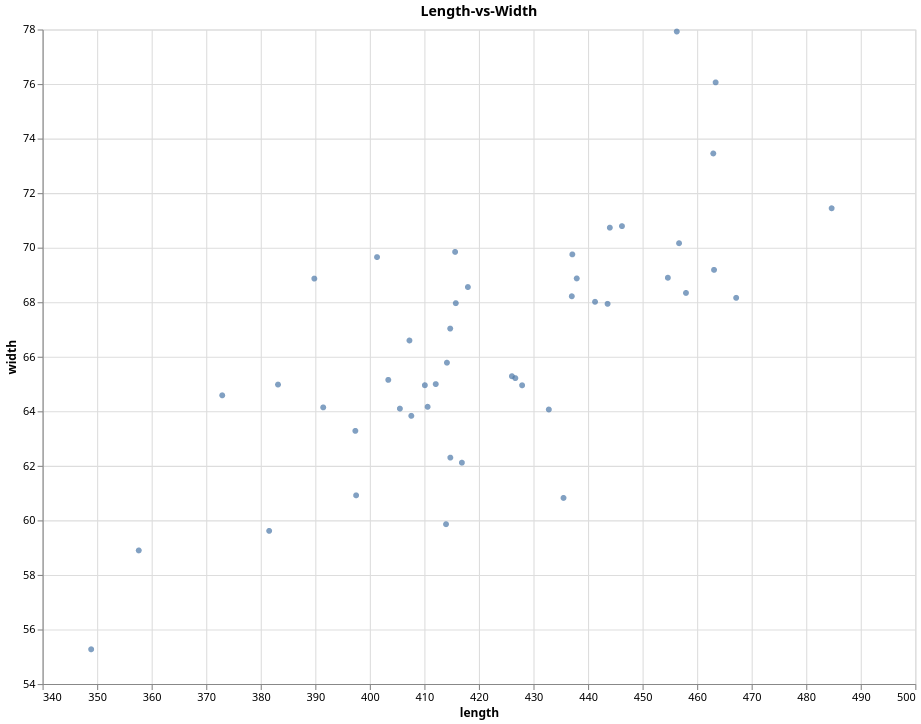
\includegraphics[scale=0.35]{screenshots/fitted_augmented_scatterplot.png}
\caption{Scatterplot of calculated length and width of 47 samples from an fitted+augmented Gaussian process.}
\label{fig:scatterplot_fitted_augmented}
\end{figure}
\begin{table}[h!]
\centering
\begin{tabular}{c|r|r}
 & Mean & Variance \\
\hline
Length & 421.85 & 851.79 \\
Width & 66.43 & 18.57
\end{tabular}
\caption{Mean and variance of length and width of 47 samples from a fitted+augmented Gaussian process.}
\label{table:mean_variance_fitted_augmented}
\end{table}

In figure \ref{fig:randomsamplefemur} we show the models capability by displaying one typical sample of the model.
\begin{figure}[h!]
\centering
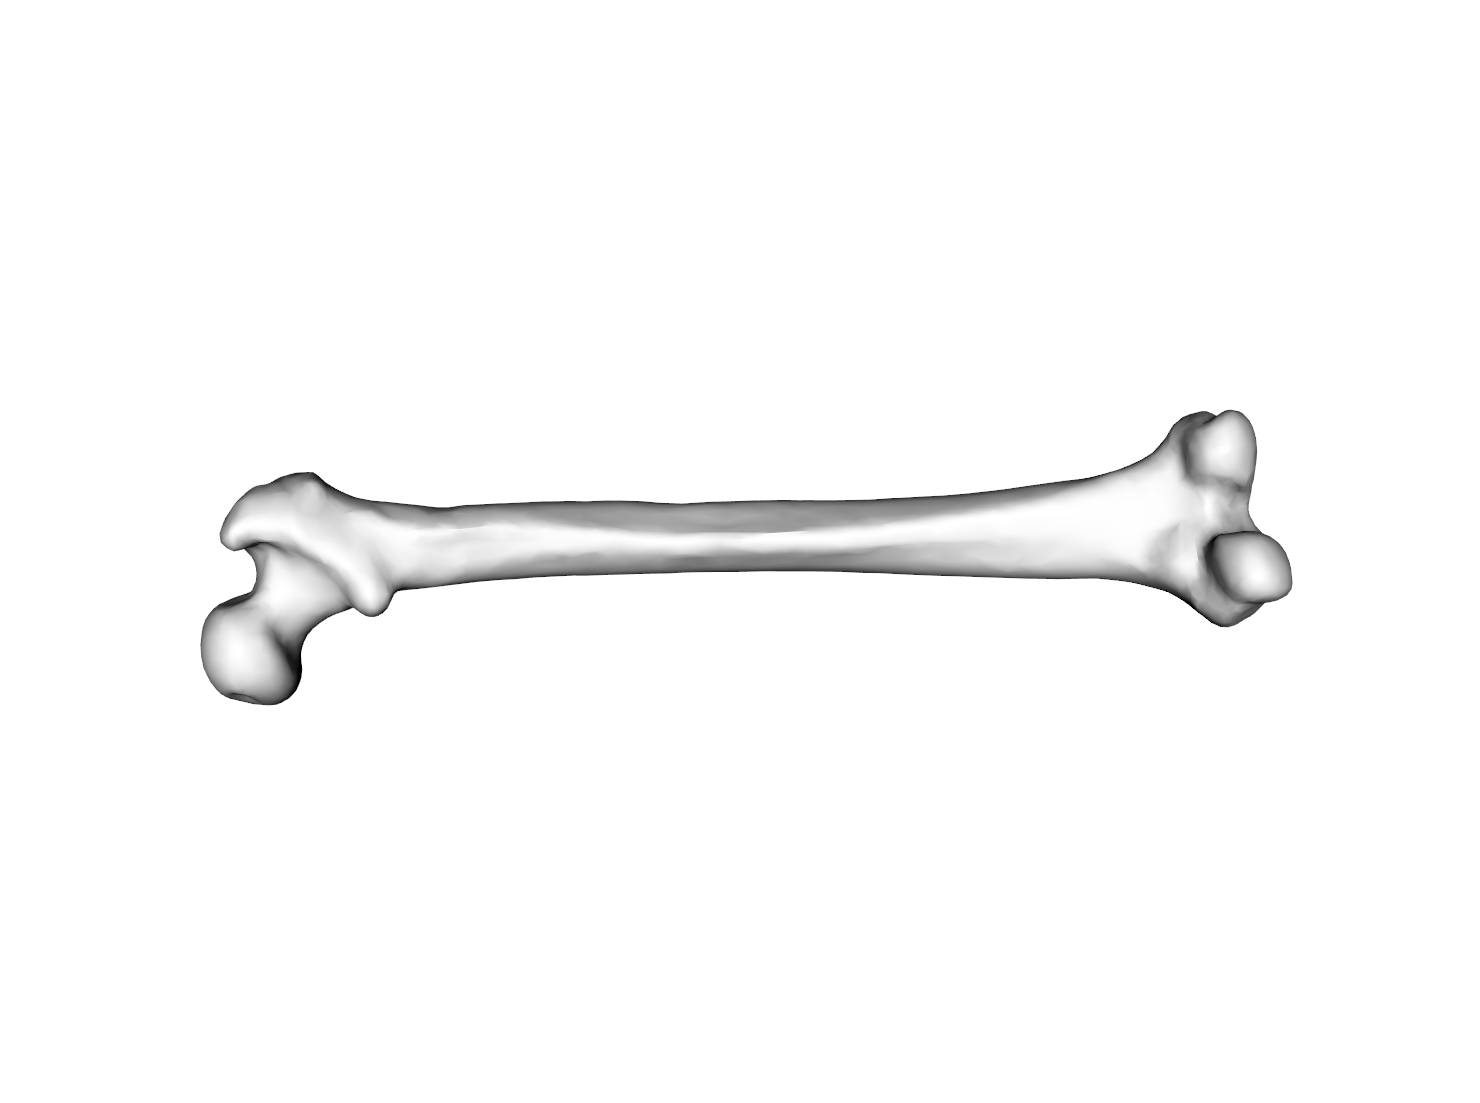
\includegraphics[scale=0.15]{screenshots/samplefemur.png}
\caption{Femur sample from final model}
\label{fig:randomsamplefemur}
\end{figure}

\newpage
\section{Conclusion}

%Add your conclusion here. What is the main result? What did you achieve, what
%needs to be done.
From the evaluation we can conclude that the model works well to generate sample femurs that have typical length and width. Further validation, for example with cross-validation, is needed to show that the model describes actual femurs well. Furthermore we notice the mean width is higher than the data mean width. This most likely stems from the fact that the original reference femur used was not an average femur. It was quite big with width $\sim 70$. Using a shape that more closely resembles an average femur to start building the model could solve this problem. Furthermore all parameters used were picked by simple trial and error and they are most likely not the optimal parameters.


\end{document}
